\section{Herstellung der ersten Platine}

\subsection{Entwurf einer Leiterplatte}
Zum Entwurf einer funktionsfähigen Platine sind ein Schaltplan, ein PCB-Layout und die passenden Bauteile mit den zugehörigen Footprints erforderlich.
Für die erste Platine werden nur Testpunkte erstellt, weshalb die Erstellung eigener Bauteile und Footprints in sogenannten Libraries nicht im Fokus stand.
Der Schwerpunkt liegt vielmehr auf der Herstellung einer spezifischen Leiterbahn auf der Platine.\\
\\
Eine besondere Anforderung bestand darin, eine Leiterbahn mit einem definierten Widerstand von genau $200,\text{m}\Omega$ zu realisieren.
Um dies zu erreichen wird eine feste Breite für die Leiterbahn vorgegeben, anhand derer die erforderliche Länge der Bahn berechnet werden muss.

\paragraph{Berechnung:} 
\begin{align*}
\text{Gegeben:} & \quad b=0{,}275\,\text{mm}, \quad R=0{,}2\,\Omega, \quad \rho=0{,}01721\,\Omega\cdot\text{mm}^2/\text{m}, \quad h=0{,}035\,\text{mm} \\ 
\text{Gesucht:} & \quad l \\ R &= \frac{\rho \cdot l}{A} \quad \Rightarrow \quad l = \frac{R \cdot b \cdot h}{\rho} \\
l &= \frac{0{,}2\,\Omega \cdot 0{,}275\,\text{mm} \cdot 0{,}035\,\text{mm}}{0{,}01721\,\Omega\cdot\text{mm}^2/\text{m}} = 111{,}85\,\text{mm} 
\end{align*}
\\
Die berechnete Länge wird anschließend in das Platinenlayout erstellt.
Da die Gesamtlänge der Leiterbahn durch das Layout die berechneten Länge überschreiten könnte, wird die Leiterbahn in einem wellenartigen Muster umgesetzt, um die geforderte Gesamtlänge einzuhalten.

\begin{figure}[h]
\centering 
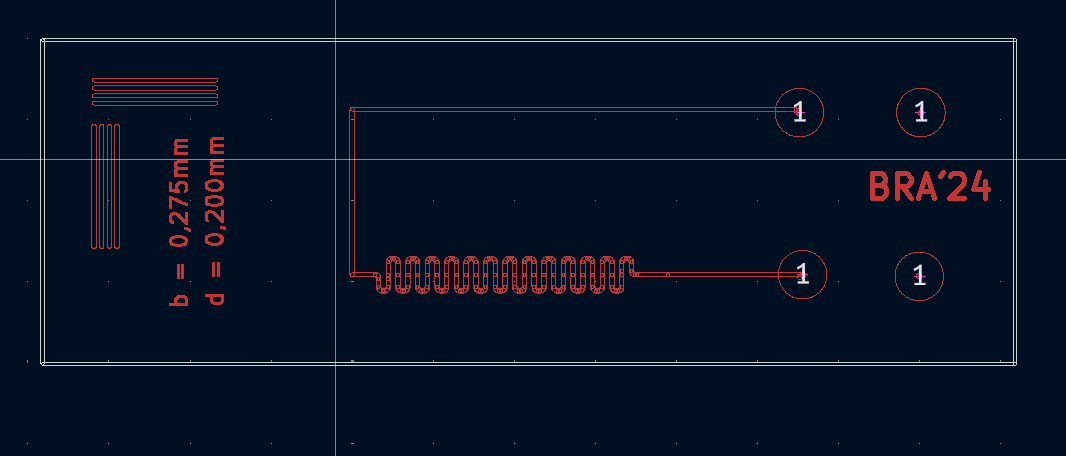
\includegraphics [width=\linewidth, height=6cm]{\figdir/PCB-Layout breite 0,275mm.png}
\caption{PCB Layout der Platine mit Leiterbahn = 0,275 mm}
\label{fig:Abbildung 1}
\end{figure}

\noindent
Außerdem wird der Name des Studierenden zusammen mit der Jahreszahl auch als Kupferbahn ausgeführt.
Bei der herkömmlichen Fertigung von Leiterplatten wird ein Bestückungsdruck für die Bezeichnungen der Komponenten und spezifischen Informationen zu den Bauteilen verwendet.
Da hier allerdings nur eine Kupferschicht vorgesehen ist, wird darauf verzichtet.
\\
Für die nachfolgende Messung bzw. Überprüfung unter dem Mikroskop werden vier Linien horizontal und vertikal in festem Abstand auf der Leiterplatte definiert.

\begin{figure}[h]
\centering 
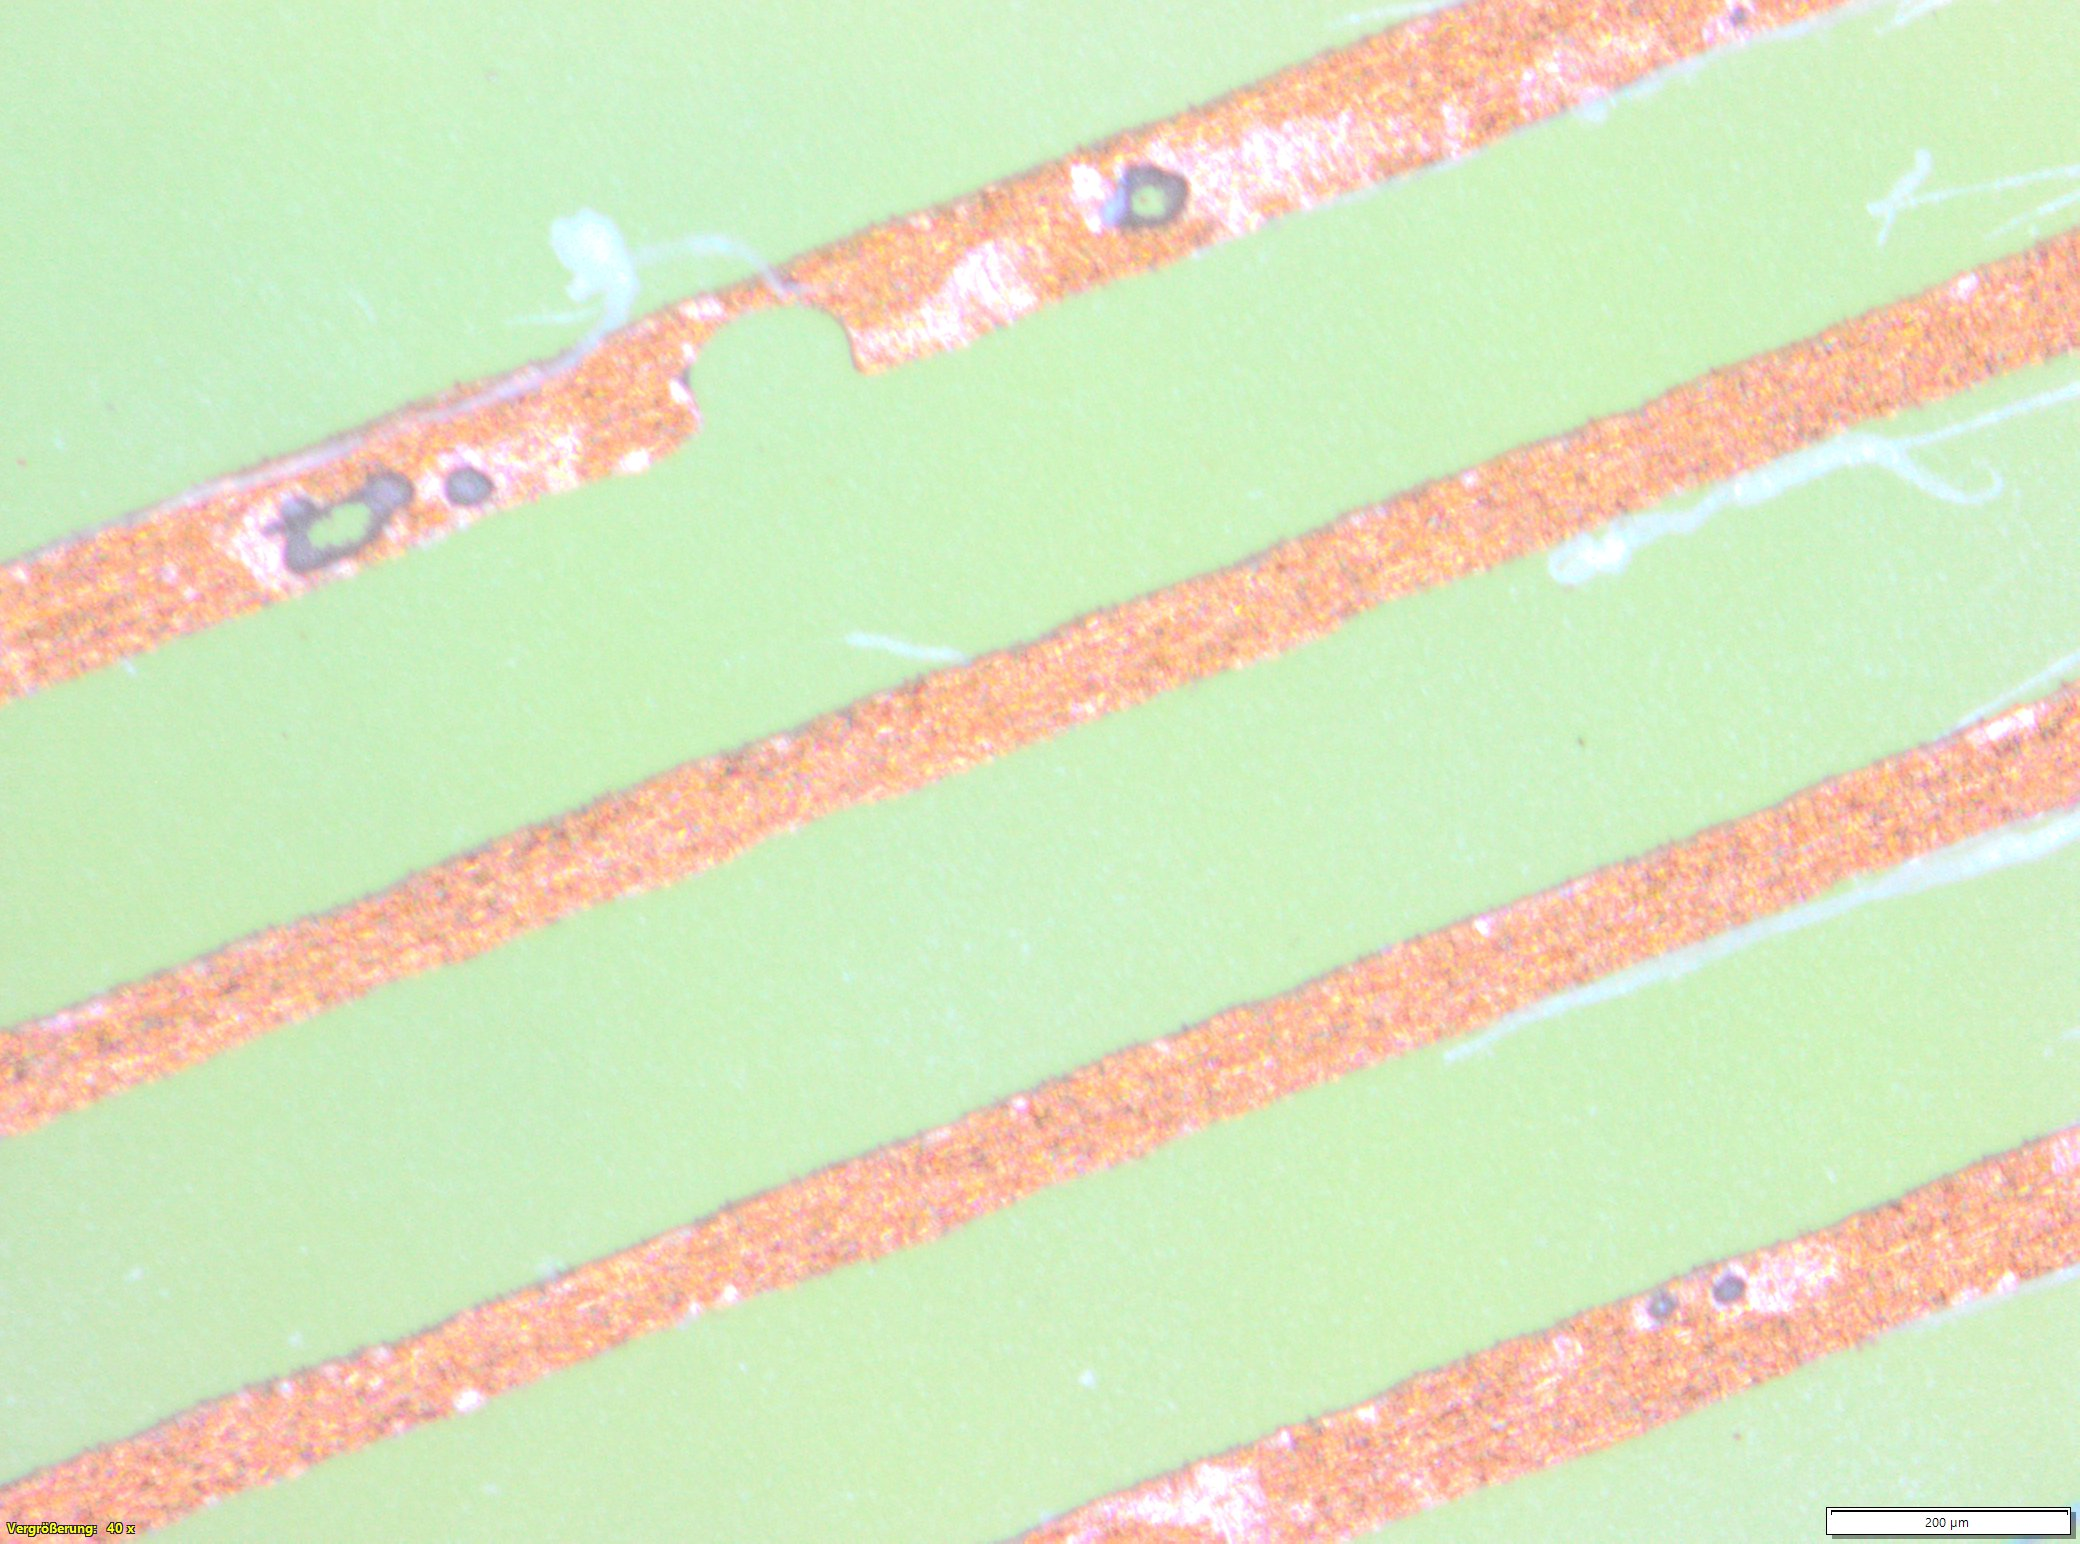
\includegraphics [width=12cm ,height=6cm]{\figdir/Mikroskopie_paralleleLeiterbahn}
\caption{parallele Leiterbahnen unter Mikroskop}
\label{fig:Abbildung 2}
\end{figure}

\noindent
Die Ursachen für Fehler auf den geätzten Leiterbahnen sind vielschichtig.
So können beispielsweise Ungenauigkeiten beim Belichten oder Staub auf der Maske zu unpräzisen Strukturen führen.
Während des Entwicklungsprozesses können ungleichmäßige Ergebnisse durch unvollständige oder fehlerhafte Abläufe entstehen.
Im Ätzprozess selbst können Probleme wie unzureichende Ätzlösung, Lufteinschlüsse, Überätzung oder ungleichmäßiger Materialabtrag auftreten.
Um derartige Fehler zu vermeiden, bedarf es einer sauberen Arbeitsumgebung sowie optimierter Prozessparameter.

\subsection{Herstellung der Platine}
Für die Herstellung von Leiterplatten existieren diverse Verfahren.
An der Hochschule wird das Ätzverfahren eingesetzt.
Dieses besteht aus den drei Hauptschritten Belichten, Entwickeln und Ätzen.
Darüber hinaus sind mehrere Vor- und Nachbearbeitungsschritte erforderlich, um eine optimale Verarbeitung zu gewährleisten.\\
\\
Um das Material effizient zu nutzen und Produktionsabfälle zu minimieren, werden mehrere Leiterplatten zu einer Einheit zusammengefasst, die als Nutzen bezeichnet wird.
Ein solcher Nutzen entspricht der Größe einer Europlatine, was eine standardisierte und platzsparende Anordnung ermöglicht.\\
\\
Die Belichtungsmaske für den Nutzen wird durch Bedrucken einer transparenten Folie mit einem Laserdrucker erstellt.
Um eine gleichmäßige Lichtundurchlässigkeit sicherzustellen, werden zwei identische Folien exakt übereinander geklebt.
Dies gewährleistet eine hohe Präzision beim Belichten und damit eine gute Qualität der späteren Leiterplatten.\\
\\
Nach dem Ätzen sind die Platinen noch als Teil des Europlatinen-Nutzens verbunden und müssen im Anschluss voneinander getrennt werden.
Der Trennvorgang erfolgt mithilfe einer Hebelschere.
Die Verwendung dieses Werkzeugs ermöglicht ein sauberes und präzises Zuschneiden der einzelnen Platinen.\\

\subsubsection{Belichten}
Beim Ätzverfahren wird die Platine mit einem Ätzresistlack versehen, der an bestimmten Stellen durch Belichtung seine Schutzfunktion verliert. Um dies zu ermöglichen, wird die auf dem Rohling befindliche Schutzfolie der Ätzresistschicht entfernt. Danach wird die Belichtungsmaske exakt auf dem Rohling positioniert.\\
\\
Damit die Belichtungsmaske während des Belichtungsvorgangs nicht verrutscht, verfügt das Belichtungsgerät über eine Vakuumfolie, die die Maske sicher auf dem Rohling fixiert. Für eine Standardleiterplatte beträgt die Belichtungsdauer etwa 2 Minuten. Während dieser Zeit bleibt der UV-Belichtungsapparat geschlossen, um eine gleichmäßige Belichtung zu gewährleisten.\\
\\
Nach der Belichtung sollte der Rohling mit der Maske etwas abkühlen, bevor die Belichtungsmaske entfernt wird. Es ist jedoch wichtig, den nächsten Schritt so schnell wie möglich durchzuführen, da das Ätzresist bei Tageslicht weiter belichtet werden kann. Dies könnte dazu führen, dass ungewollte Bereiche ihre Schutzwirkung verlieren und Fehler im weiteren Herstellungsprozess auftreten.

\begin{figure}[h]
\centering 
\includegraphics [width=12cm ,height=5.5cm]{\figdir/Belichtungsmaske und Gerät}
\caption{Belichtungsmaske und Gerät}
\label{fig:Abbildung 3}
\end{figure}

\subsubsection{Entwickeln}
Im Rahmen des Entwicklungsprozesses der Platine wird diese zunächst in einen Rahmen eingespannt und in eine Kammer gebracht, in der sie mit einer Lösung von Natriumhydroxid besprüht wird.
Das Besprühen ist auf etwa eine Minute zu beschränken, wobei bereits nach 15 bis 20 Sekunden erste Ergebnisse sichtbar sein sollten.\\
\\
Nach Ablauf der Minute wird der Entwicklungsprozess durch Erhitzen in einem Wasserbad gestoppt.
Im Anschluss werden die verbliebenen Rückstände unter fließendem Wasser abgespült, um eine vollständige Reinigung der Oberfläche zu gewährleisten.\\
\\
Nach diesem Schritt sollten die ungeschützten Kupferflächen sichtbar werden, die im darauffolgenden Prozess durch Ätzen entfernt werden.\\
Für ein fehlerfreies Ergebnis ist es entscheidend, dass die Natronlauge frisch, leicht erhitzt und im korrekten Mischverhältnis verwendet wird.\\

\begin{figure}[h]
\centering 
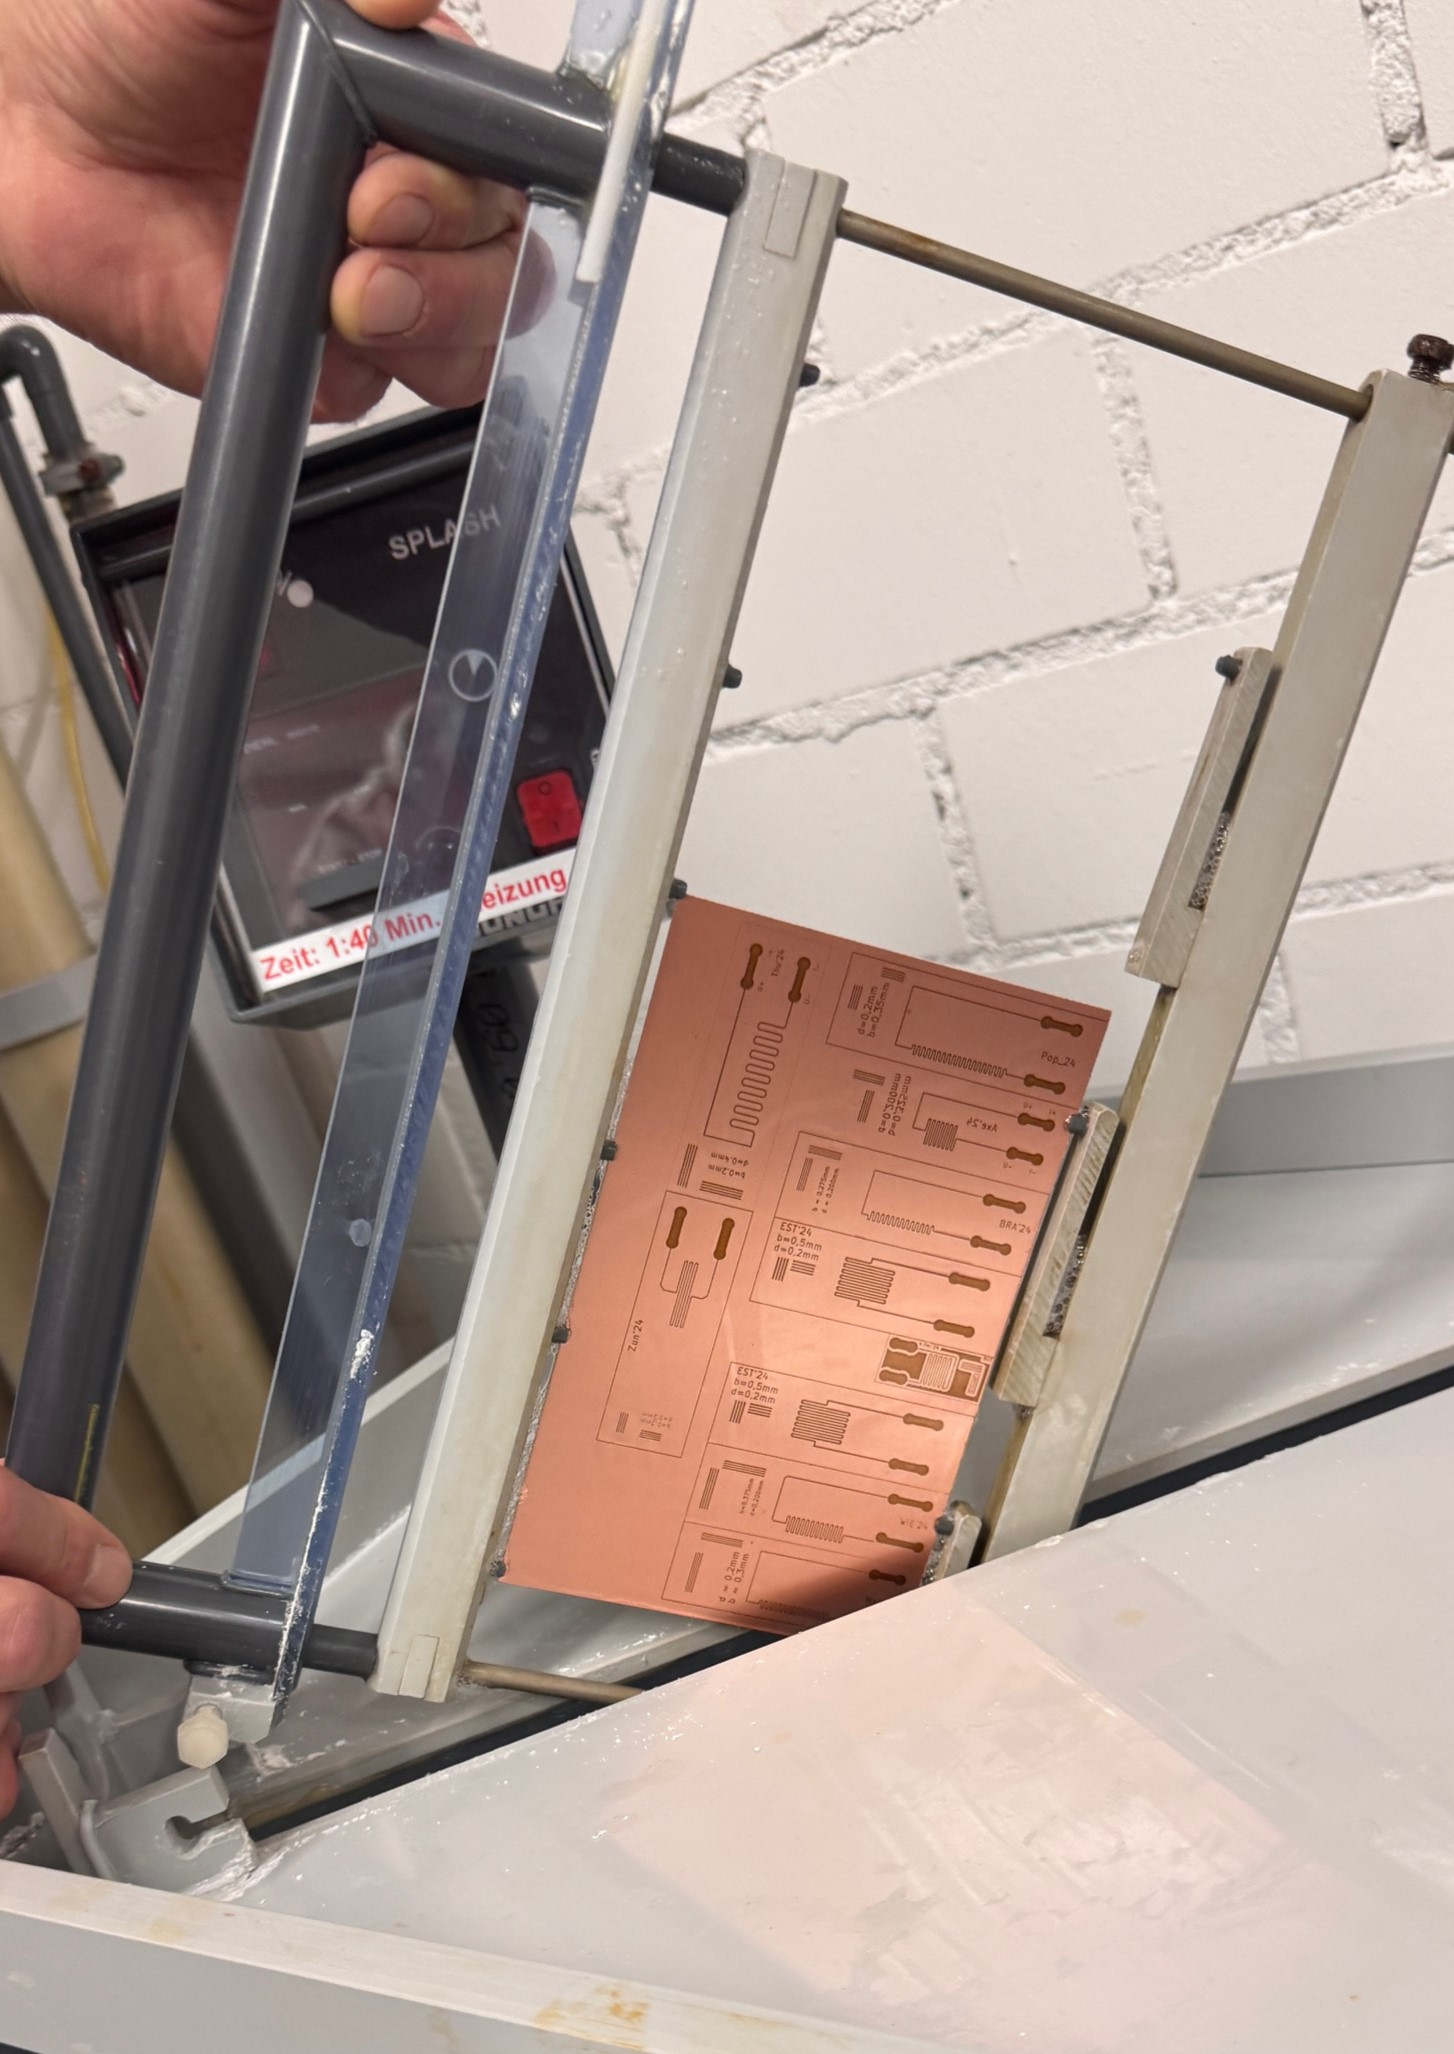
\includegraphics [width=12cm ,height=8cm]{\figdir/Leiterbahn nach Entwickeln}
\caption{Leiterbahn nach Entwickeln}
\label{fig:Abbildung 4}
\end{figure}

\subsubsection{Ätzen}
Für den Ätzvorgang wird die Platine erneut in einen Rahmen eingespannt und in einer Kammer mit Eisen-III-Chlorid-Lösung besprüht.
Die Ätzdauer beträgt ca. 3 Minuten, wobei die ungeschützten Kupferbereiche gezielt vom Ätzmittel entfernt werden.
Im Anschluss wird die Platine in einem Wasserbad vor gereinigt, um verbleibende Rückstände des verwendeten Ätzmittels zu entfernen.
Abschließend wird die Platine unter fließendem Wasser gründlich abgespült.
Dazu wird die Leiterplatte noch getrocknet und für die weitere Verarbeitung vorbereitet.\\
\\
Während des Ätzvorgangs können jedoch Fehler aus dem Entwicklungsprozess sichtbar werden.
Ein unzureichend entwickeltes Ätzresist zeigt sich daran, dass die Kupferschichten nach den ersten 30 Sekunden nicht die typische hellrosa Verfärbung aufweisen.
Dies kann auf eine unzureichende Auftragung oder eine fehlerhafte Entwicklung des Resists zurückzuführen sein, was wiederum ungewollten Materialabtrag und fehlerhafte Leiterbahnen zur Folge haben kann.

\subsubsection{Nachbearbeitung}
Nach dem Ätzen erfolgt das Bohren der Löcher in die Platine.
Dabei entsteht Epoxidharzstaub, der als gesundheitsschädlich und potenziell krebserregend einzustufen ist.
Um die Belastung durch diesen Staub zu vermeiden, ist der Einsatz einer effektiven Absaugung zwingend erforderlich.
In diesem Praktikum wurde dieser Bearbeitungsschritt ausgelassen, da keine funktionalen Leiterplatten hergestellt wurden.\\
\\
Nach Abschluss dieses Prozesses kann die Leiterplatte mit Bauteilen bestückt und verlötet werden.
Für die erste Platine werden hierbei lediglich Testpunkte aufgelötet, um die Funktionsfähigkeit zu überprüfen.
Abschließend wird die Leiterplatte durch das Auftragen eines Schutzlacks vor Korrosion geschützt.
Auch diese Schritte wurden im Rahmen des Praktikums nicht durchgeführt.
